% Native editable composition from verified, unchanged IDE images.
\par
\begin{figure}[htbp]
  \centering
  \sbox0{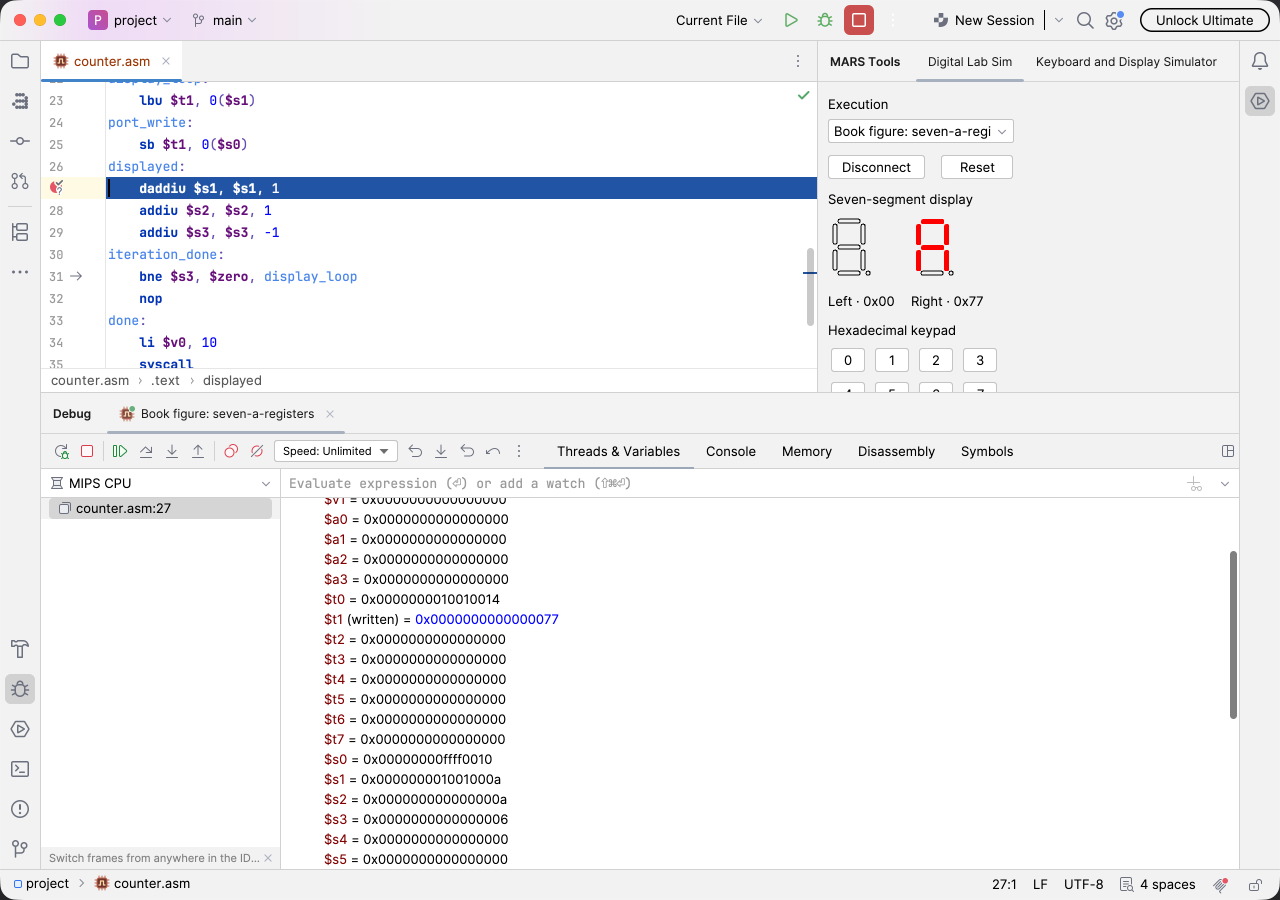
\includegraphics[artifact]{packages/005-seven-segment-counter/captures/f03-a-glyph/registers.png}}
  \sbox2{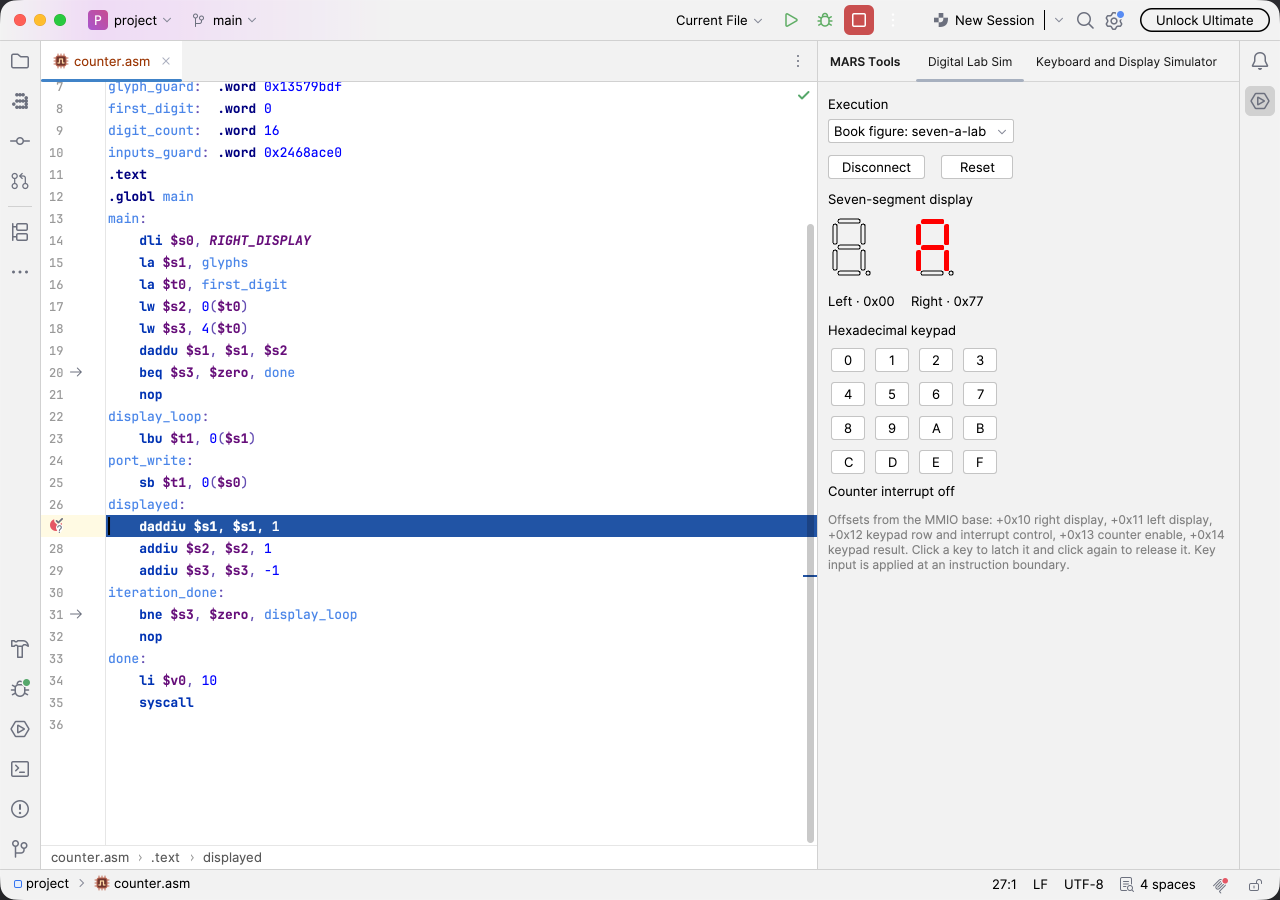
\includegraphics[artifact]{packages/005-seven-segment-counter/captures/f03-a-glyph/lab.png}}
  \edef\MARSasourceLeft{\the\dimexpr0.036718750\wd0\relax}
  \edef\MARSasourceBottom{\the\dimexpr0.774444444\ht0\relax}
  \edef\MARSasourceRight{\the\dimexpr0.611718750\wd0\relax}
  \edef\MARSasourceTop{\the\dimexpr0.147777778\ht0\relax}
  \edef\MARSalabLeft{\the\dimexpr0.643750000\wd2\relax}
  \edef\MARSalabBottom{\the\dimexpr0.652222222\ht2\relax}
  \edef\MARSalabRight{\the\dimexpr0.228906250\wd2\relax}
  \edef\MARSalabTop{\the\dimexpr0.213333333\ht2\relax}
  \edef\MARSaregistersLeft{\the\dimexpr0.246093750\wd0\relax}
  \edef\MARSaregistersBottom{\the\dimexpr0.075555556\ht0\relax}
  \edef\MARSaregistersRight{\the\dimexpr0.557812500\wd0\relax}
  \edef\MARSaregistersTop{\the\dimexpr0.673333333\ht0\relax}
  \begin{tikzpicture}[alt={Three annotated details at displayed with native breakpoint condition s2 equals ten. The next instruction advances the glyph pointer. The left display is blank with mask 00 and the right shows A with mask 77, decimal point off. Registers t1, s2 and s3 contain hexadecimal 77, decimal ten and decimal six.}]
    \node[anchor=north west,inner sep=0,font=\small\bfseries] (source-title) at (6mm,0) {Use the same boundary on iteration eleven};
    \node[anchor=north west,inner sep=0] (source) at ([yshift=-1mm]source-title.south west) {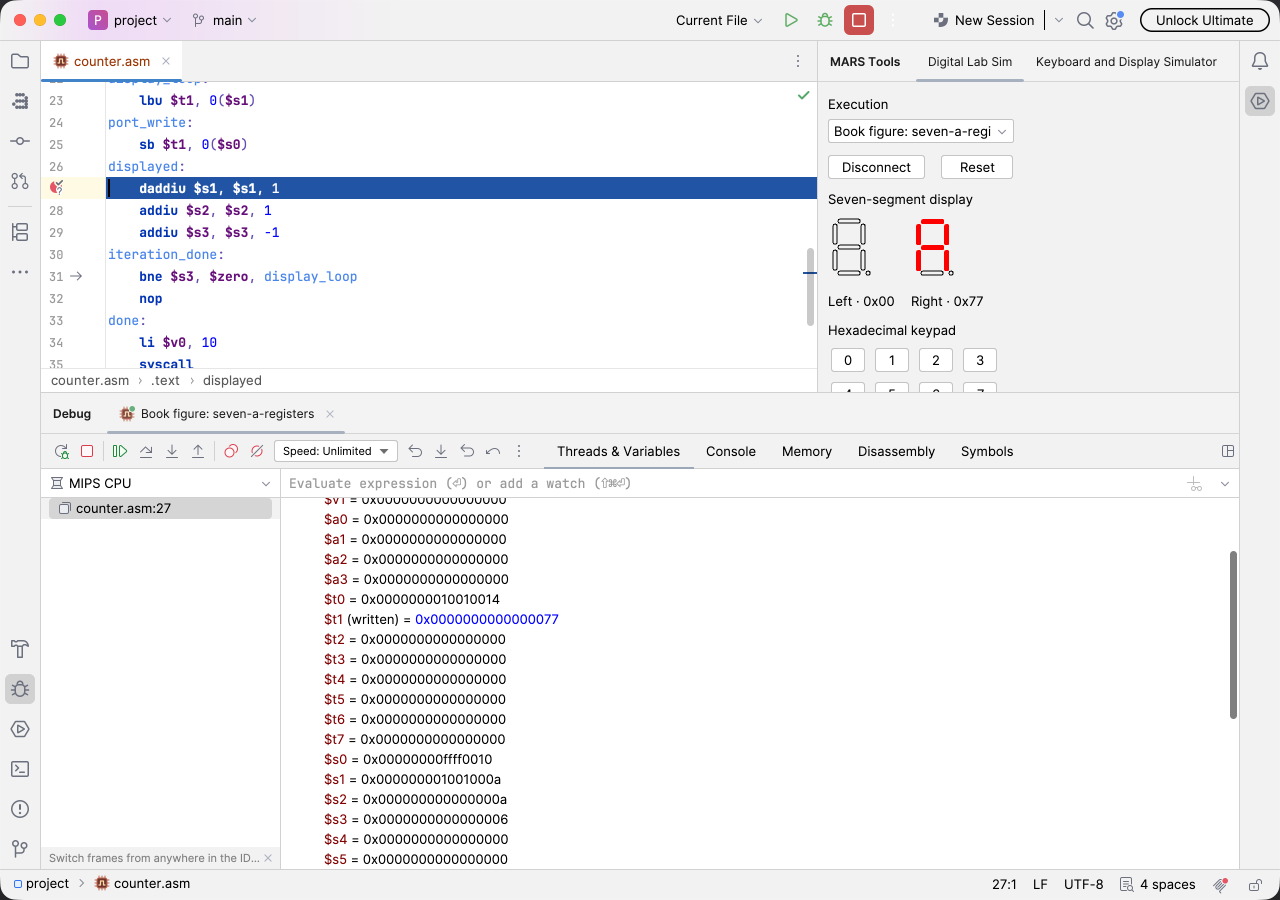
\includegraphics[width=0.7\linewidth,artifact,trim={\MARSasourceLeft{} \MARSasourceBottom{} \MARSasourceRight{} \MARSasourceTop{}},clip]{packages/005-seven-segment-counter/captures/f03-a-glyph/registers.png}};
    \begin{scope}[shift={(source.south west)},x={($(source.south east)-(source.south west)$)},y={($(source.north west)-(source.south west)$)}]
      \draw[black,line width=0.7pt] (0.135555556,0.057142857) rectangle (0.515555556,0.371428571);
      \node[draw=black,fill=white,circle,inner sep=1.5pt,font=\footnotesize] at ($(0.135555556,0.371428571)+(-3mm,0)$) {1};
    \end{scope}
    \node[anchor=north west,inner sep=0,font=\small\bfseries] (lab-title) at ([yshift=-2mm]source.south west) {The table supplies the shape of A};
    \node[anchor=north west,inner sep=0] (lab) at ([yshift=-1mm]lab-title.south west) {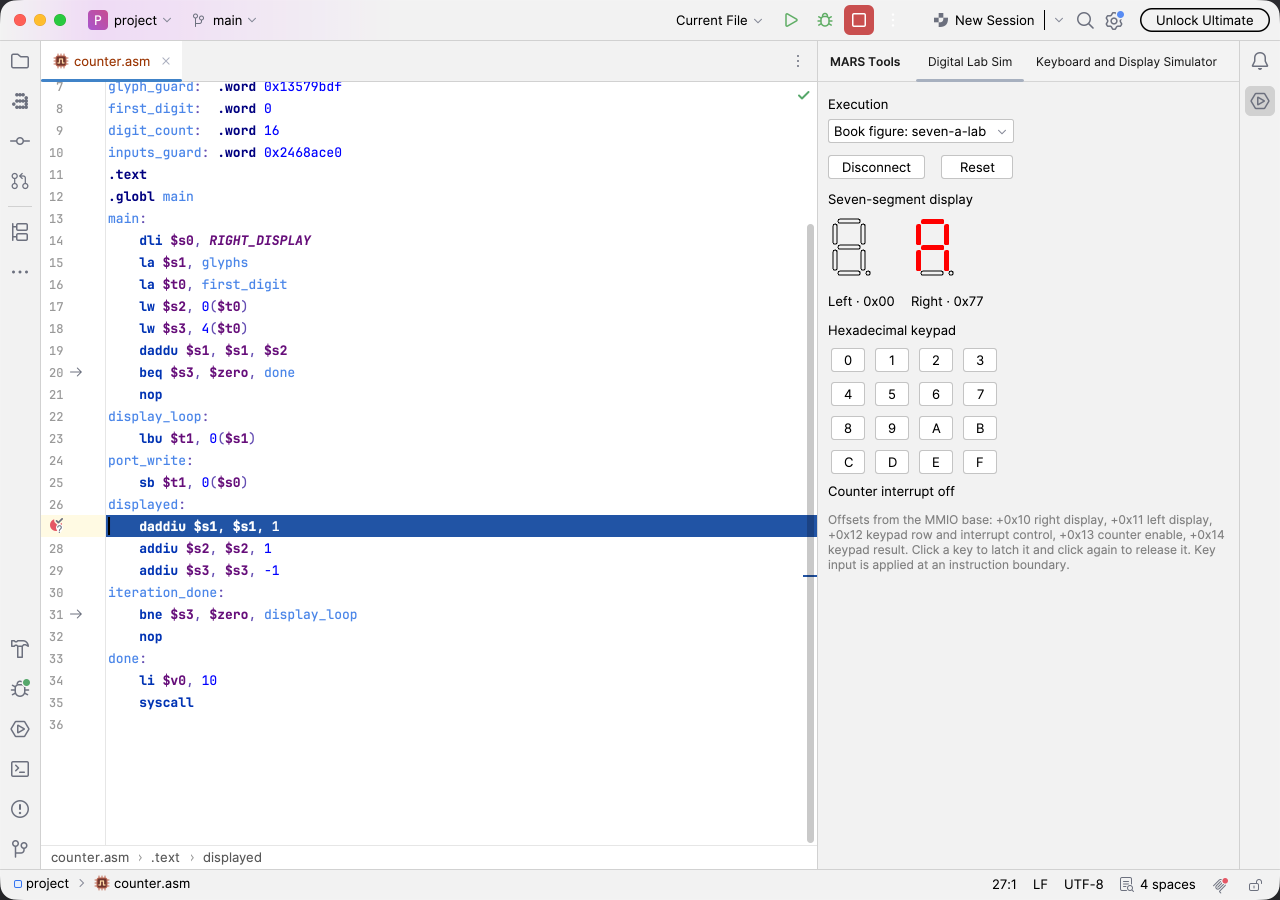
\includegraphics[width=0.34\linewidth,artifact,trim={\MARSalabLeft{} \MARSalabBottom{} \MARSalabRight{} \MARSalabTop{}},clip]{packages/005-seven-segment-counter/captures/f03-a-glyph/lab.png}};
    \begin{scope}[shift={(lab.south west)},x={($(lab.south east)-(lab.south west)$)},y={($(lab.north west)-(lab.south west)$)}]
      \draw[black,line width=0.7pt] (0.024539877,0.214876033) rectangle (0.815950920,0.818181818);
      \node[draw=black,fill=white,circle,inner sep=1.5pt,font=\footnotesize] at ($(0.024539877,0.818181818)+(-3mm,0)$) {2};
    \end{scope}
    \node[anchor=north west,inner sep=0,font=\small\bfseries] (registers-title) at ([yshift=-2mm]lab.south west) {The index is ten; the glyph byte is 119};
    \node[anchor=north west,inner sep=0] (registers) at ([yshift=-1mm]registers-title.south west) {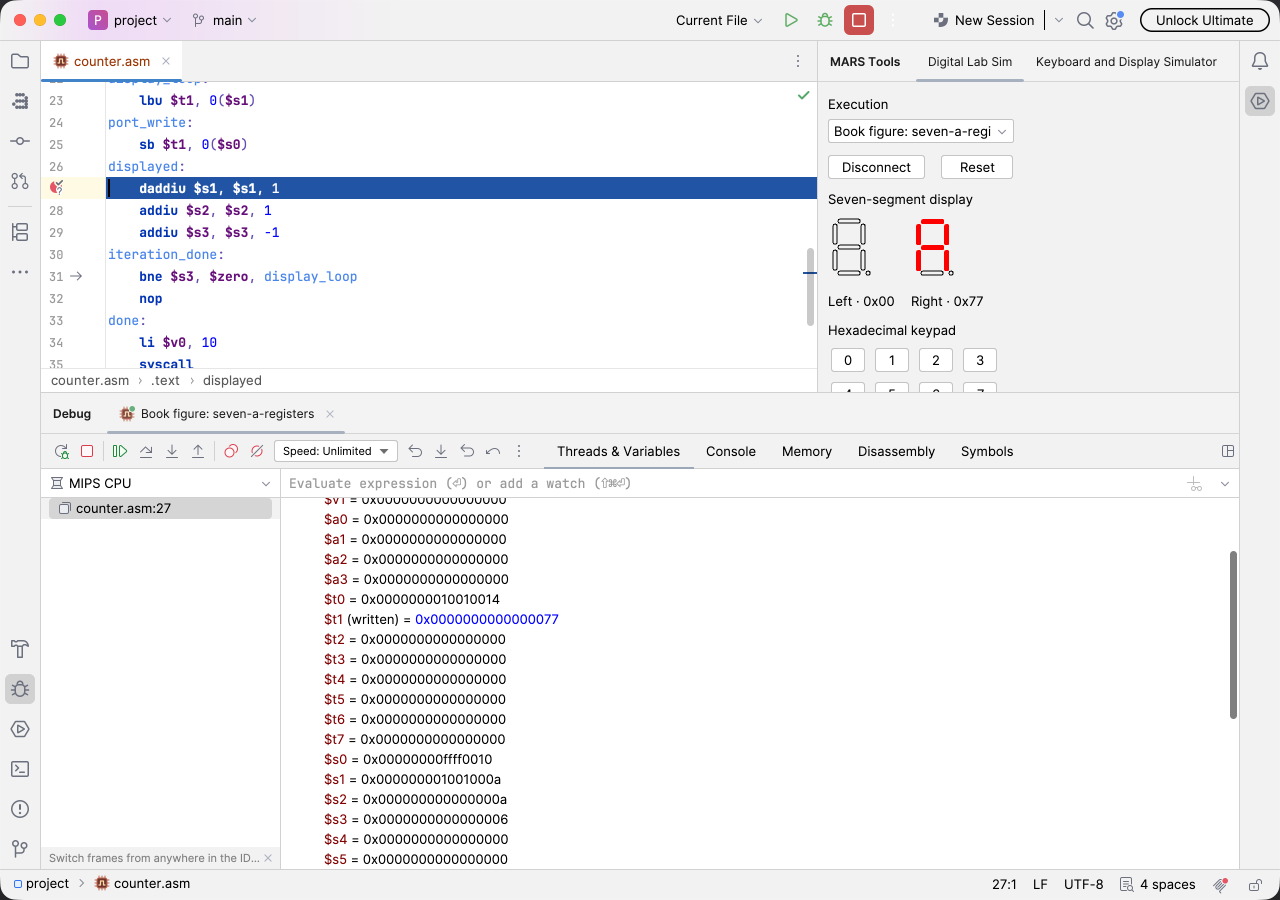
\includegraphics[width=0.43\linewidth,artifact,trim={\MARSaregistersLeft{} \MARSaregistersBottom{} \MARSaregistersRight{} \MARSaregistersTop{}},clip]{packages/005-seven-segment-counter/captures/f03-a-glyph/registers.png}};
    \begin{scope}[shift={(registers.south west)},x={($(registers.south east)-(registers.south west)$)},y={($(registers.north west)-(registers.south west)$)}]
      \draw[black,line width=0.7pt] (0.023904382,0.013274336) rectangle (0.976095618,0.986725664);
      \node[draw=black,fill=white,circle,inner sep=1.5pt,font=\footnotesize] at ($(0.023904382,0.986725664)+(-3mm,0)$) {3};
    \end{scope}
  \end{tikzpicture}
  \par\smallskip
  \begin{minipage}{\linewidth}
    \small
    \begin{enumerate}
      \item The capture uses a native breakpoint at \texttt{displayed} with condition \texttt{\$s2 == 10}. Entries zero through nine have already been sent. The current store has completed, but the highlighted pointer update and the two counter updates have not.
      \item The right display holds \texttt{0x77}. That mask lights the segments of A while leaving the bottom segment and decimal point off. The left mask is still \texttt{0x00}. The transaction check requires the exact eleven-byte prefix ending in \texttt{0x77}, rather than accepting only a matching final picture.
      \item \texttt{\$t1}=\texttt{0x77}=119 is the glyph mask; \texttt{\$s2}=\texttt{0x0a}=10 is its table index. \texttt{\$s3}=6 counts this iteration and the five that follow because its decrement has not executed. Keeping the index distinct from the mask prevents sending \texttt{0x0a} to the port by mistake.
    \end{enumerate}
  \end{minipage}
  \caption{The eleventh displayed boundary shows A, table entry ten. A native breakpoint condition selects this iteration.}
  \label{capture:005-seven-segment-counter-f03-a-glyph}
\end{figure}
\par
